\section{Linux Distributions}

\begin{frame}
   {Components of a Distribution}

   \begin{itemize}
      \item \textbf{Linux} Kernel
      \item Tools for:
      \begin{itemize}
         \item File-related operations
         \item User management
         \item Software package management
      \end{itemize}
      \item Graphical environment
      \item Optional software packages
   \end{itemize}

\end{frame}

\cprotect\note{

   Strictly speaking, \textbf{Linux} is only the
   kernel: the core of a computer operating system.  A full
   \textbf{Linux} distribution consists of the kernel plus
   a number of other software tools, each of which provides
   a small part of the complete system.  Each tool is its
   own separate project, with its own developers working to
   perfect that piece of the system.

   Examples of separate tools include the \textbf{C/C++}
   compiler, the core system application programming
   interface, the system for drawing graphics on the
   screen, and the system for installing and updating other
components (including the kernel itself).  }

\begin{frame}
   {Linux Distribution Components}

   \begin{figure}[H]
      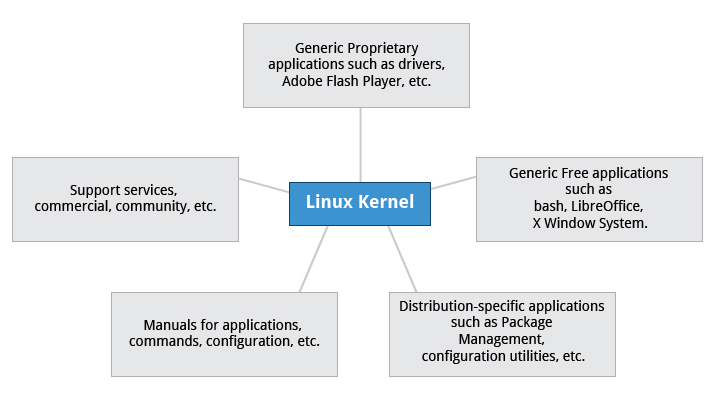
\includegraphics[height=3.2in]{IMAGES/ldistro}
      \caption{Linux Distribution Components}
   \end{figure}
\end{frame}

\cprotect\note{

   The current \textbf{Linux} kernel, along with earlier
   release versions be found at \url{www.kernel.org}.
   Usually, the various \textbf{Linux} distributions may be based on
   different kernel versions.  For example, the very popular
   \textbf{RHEL 7} distribution is based on the \textbf{3.10}
   \textbf{Linux}, which is not new , but is extremely
   stable.

   Other distributions may move more quickly in
   adopting the latest kernel releases. It is important to note
   that the kernel is not an all or nothing proposition, for
   example, \textbf{RHEL 7} and \textbf{CentOS 7} have incorporated many of the
   more recent kernel improvements into their older version
   as do  recent \textbf{Ubuntu}, \textbf{openSUSE}, \textbf{SLES} etc.

   Examples of other essential tools and ingredients provided
   by distributions include the \textbf{C/C++} compiler, the \textbf{gdb}
   debugger, the core system libraries applications need to
   link with in order to run, the low-level interface for
   drawing graphics on the screen, as well as the higher-level
   desktop environment, and the system for installing and
   updating the various components, including the kernel
itself.  }

\begin{frame}
   {Distribution Families}

   \begin{figure}[H]
      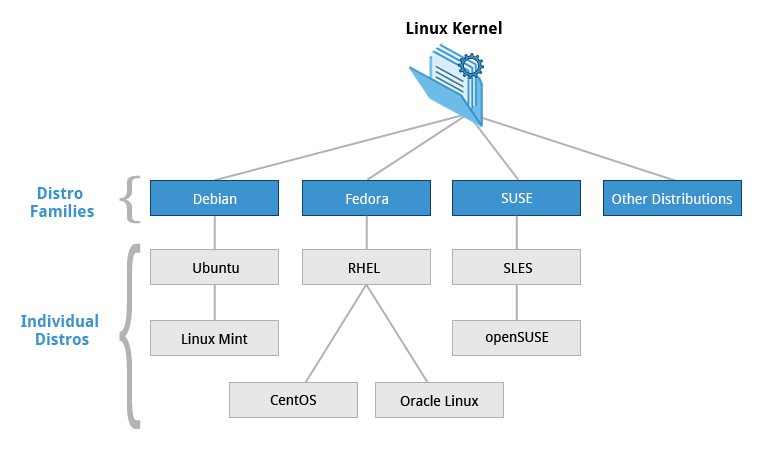
\includegraphics[scale=0.52]{IMAGES/distros}
      \caption{Linux Distribution Families}
   \end{figure}

\end{frame}

\cprotect\note {

   While there is almost an infinite variety of
   distributions (see \url{http://lwn.net/Distributions})
   most people use members of the three main families as
   diagrammed above.

}



\begin{frame}
   {Services Associated With Distributions}

   \begin{itemize}
      \item Amalgamation
      \begin{itemize}
         \item Gather up and integrate all important components
         \item Resolve conflicts, package coherently
         \item Work with upstream developers and help contribute
         patches and development
      \end{itemize}
      \item Support
      \begin{itemize}
         \item Free Internet-based support (forums, online
         documents, bug and knowledge databases)
         \item Commercial technical support
      \end{itemize}
      \item Updates (in timely fashion)
      \begin{itemize}
         \item Security and stability fixes
         \item Feature enhancements
      \end{itemize}
      \item Hardware and software certification
   \end{itemize}

\end{frame}

\cprotect\note{

   There is a vast variety of \textbf{Linux} distributions
   that cater to different audiences and organizations
   depending on their specific needs.

   Large commercial organizations tend to favor the
   so-called {Enterprise} distributions from \textbf{Red
      Hat} and \textbf{SUSE}.

   \textbf{CentOS} is a popular free alternative to
   \textbf{Red Hat Enterprise Linux} (\textbf{RHEL}).
   \textbf{Scientific Linux} is favored by the scientific
   research community for its choice of scientific and
   mathematical software packages, and is also based on
   \textbf{RHEL}.

   The \textbf{Debian} distribution is the basis of
   \textbf{Ubuntu}, \textbf{Mint Linux} and many other
   derivatives.  In particular, \textbf{Ubuntu} is very
   widely-used as it is seen as easy to learn and use, and
   has periodic \textbf{LTS} (\textbf{L}ong \textbf{T}erm
   \textbf{S}upport) releases.

   \textbf{Fedora} is community-supported and closely
   related to \textbf{RHEL}; it can be thought of as the
   development base for \textbf{RHEL}.  \textbf{openSUSE}
   plays a similar role for \textbf{SUSE}.

   Many commercial distributors, including \textbf{Red
      Hat}, \textbf{Ubuntu}, \textbf{SUSE}, and
   \textbf{Oracle}, provide commercial support for their
   distributions, as well as hardware and software
   certification.  All major distributors offer essential
   update services for keeping your system current with the
   latest security patches, bug fixes, and enhancements,
   as well as provide online support.

}



